% Copyright 2020 by Robert Hildebrand
%This work is licensed under a
%Creative Commons Attribution-ShareAlike 4.0 International License (CC BY-SA 4.0)
%See http://creativecommons.org/licenses/by-sa/4.0/

%\section{MINLP}

\section{Polynomial Optimization - Algebraic Techniques}

\section{Cylindrical Algebraic Decomposition}


\section{Gr\"obner Bases}

\section{Quantifier Elimination and Semi-algebraic Sets}

\begin{theorem}{}{}
Any alternating quantifier set can be recast as a semi-algebraic set.
\end{theorem}

\section{Polynomial Optimization}

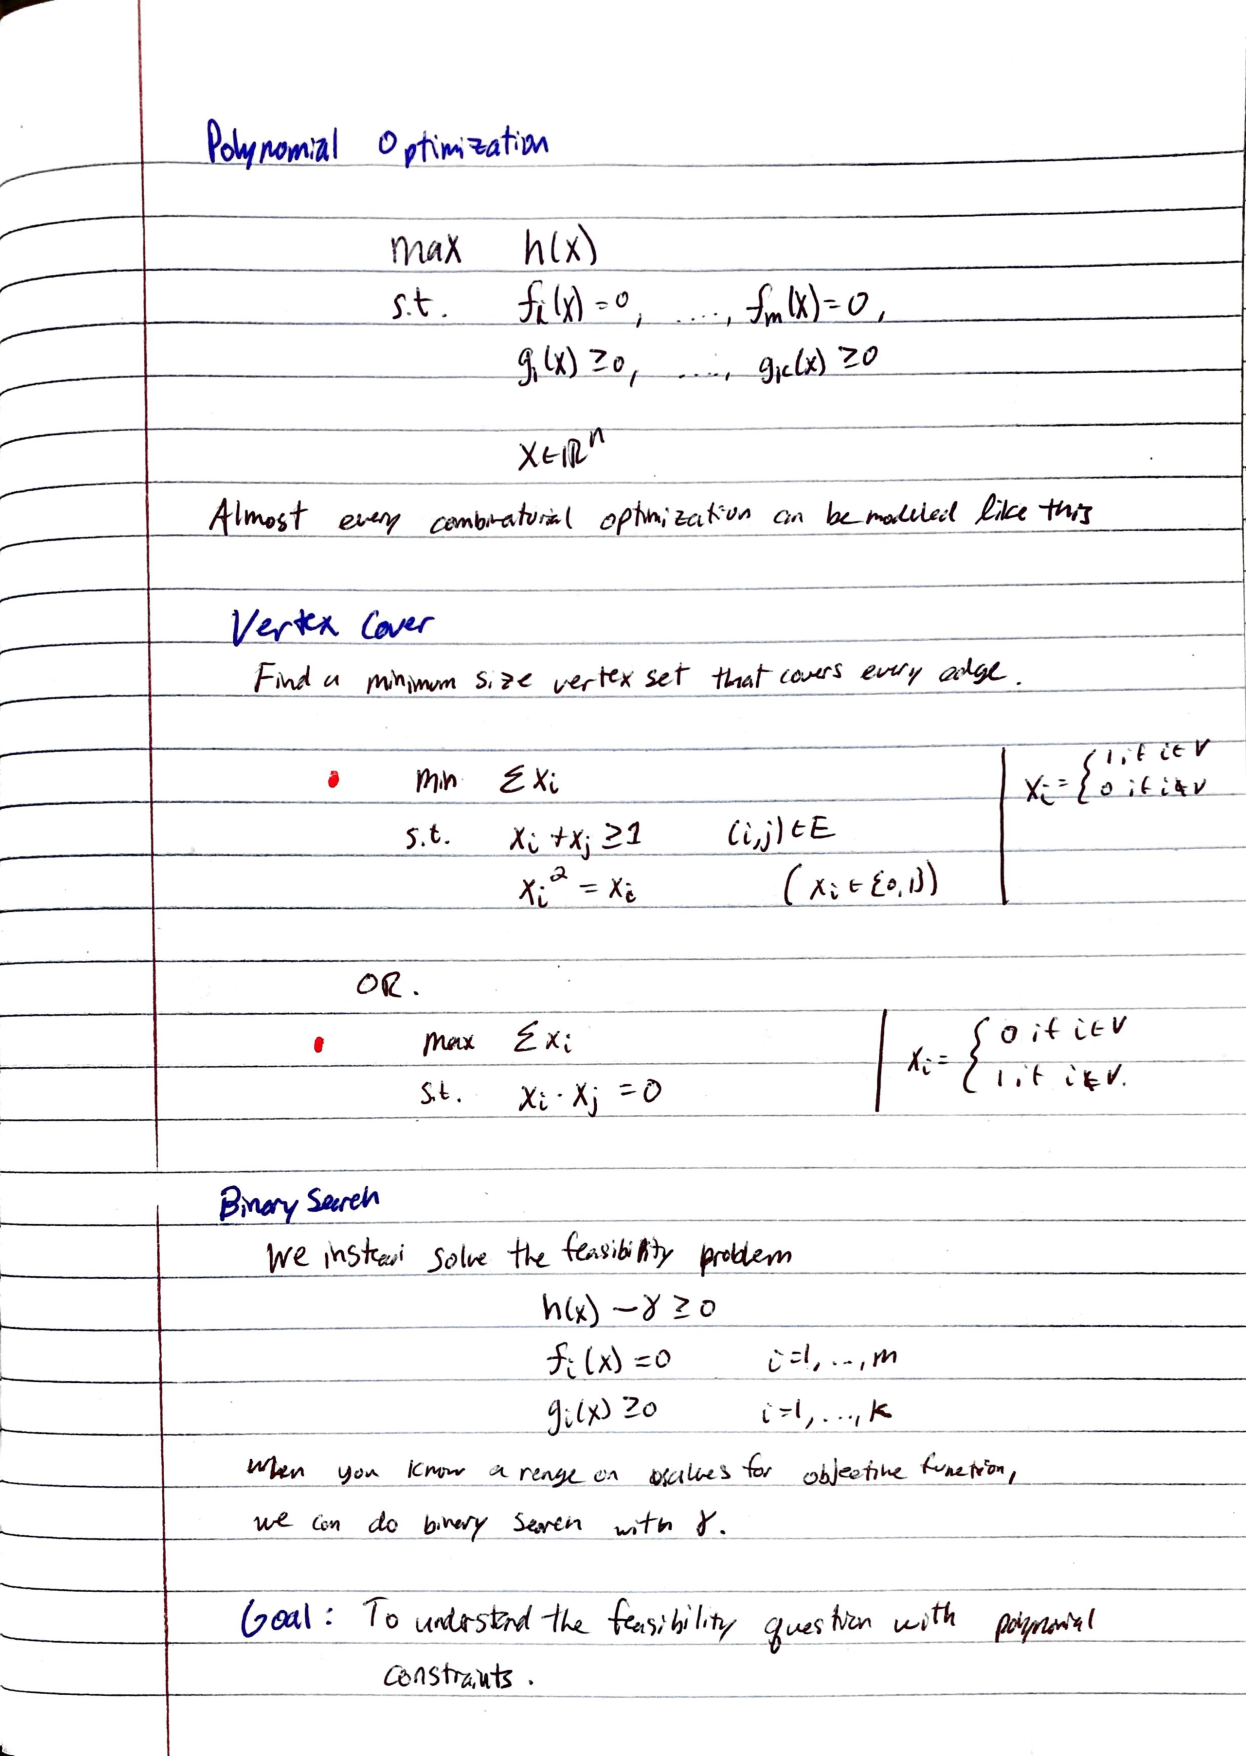
\includepdf[pages = {1,2,3,4}]{optimization/ucdavis-polynomial-optimization}
\subsection{Sums of Squares}
\includepdf[pages = {1,2,3,4,5,6,7,8,9,10,11}]{optimization/ucdavis-semidefinite-programming-SOS}
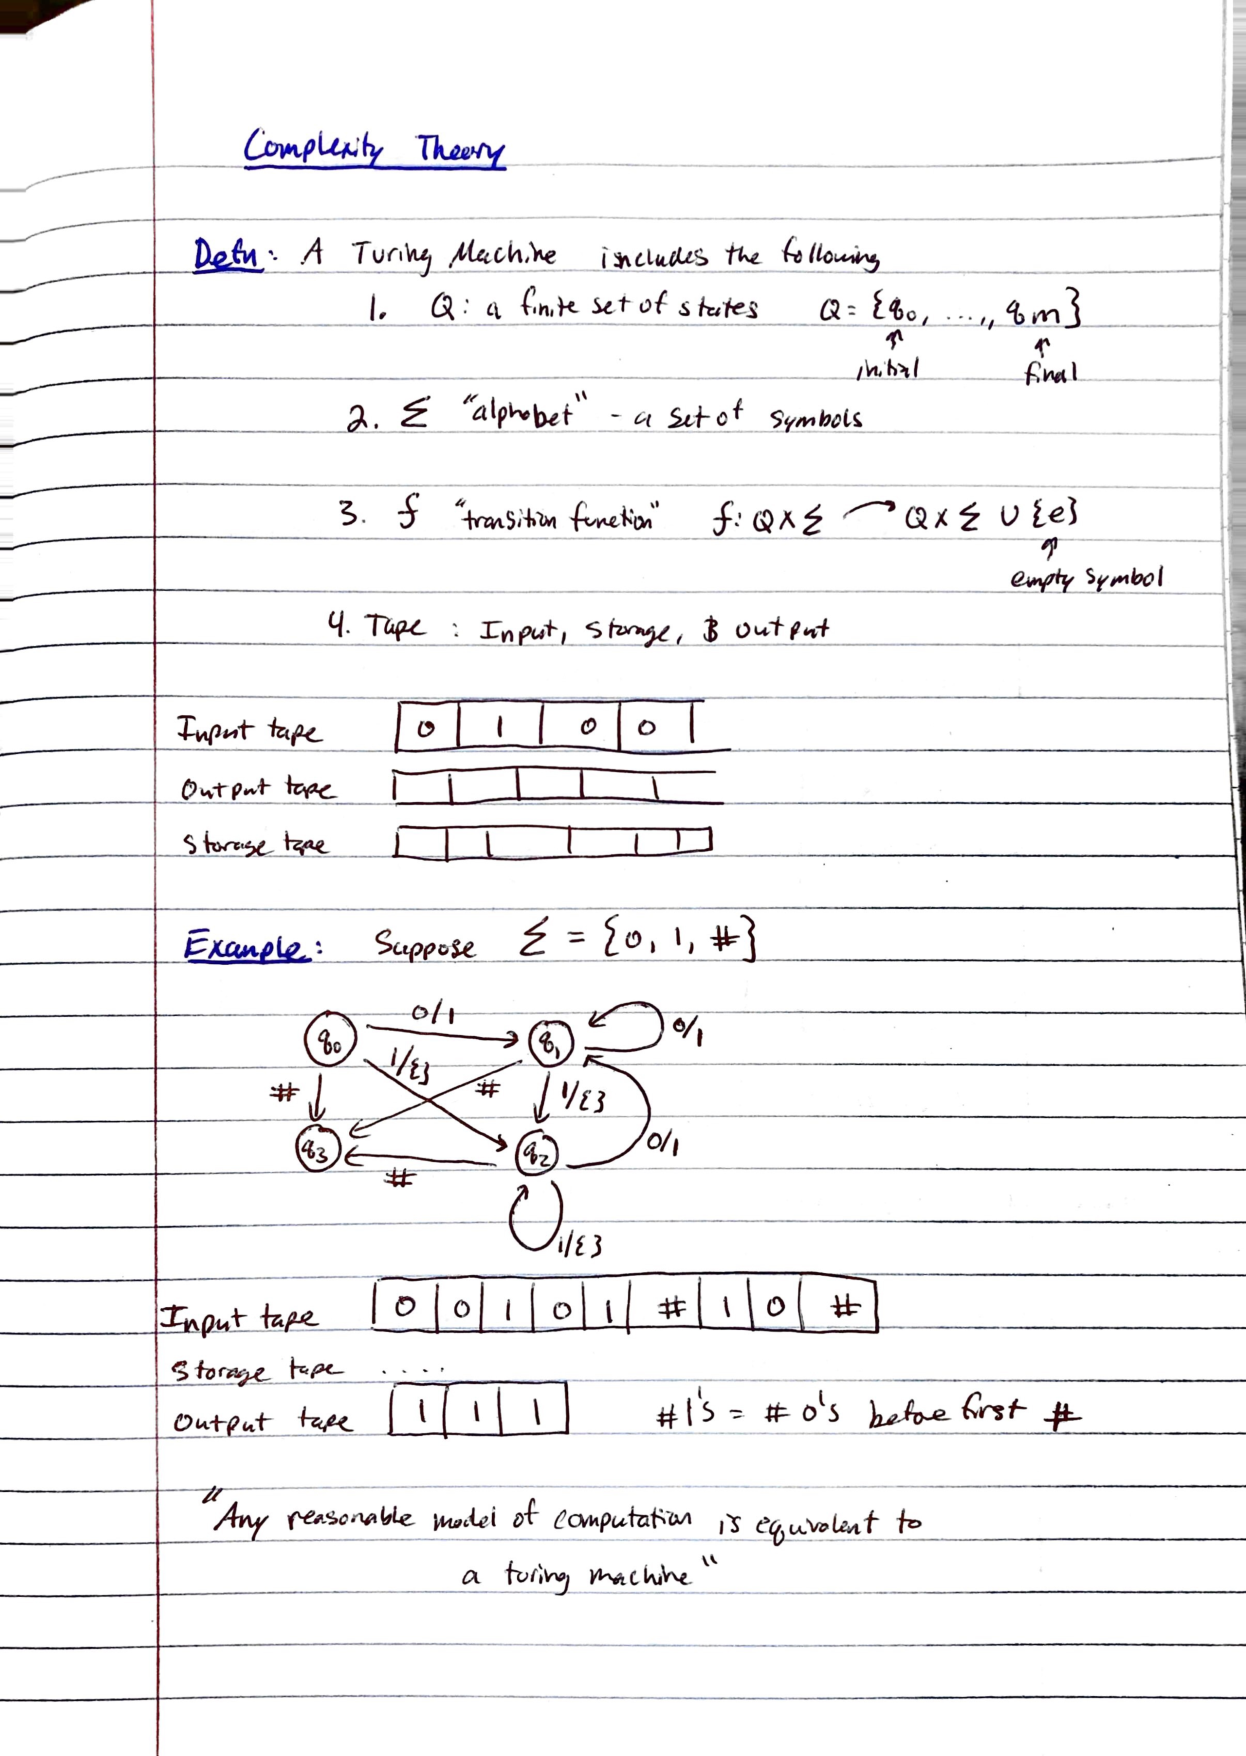
\includepdf[pages = {1,2,3,4,5}]{optimization/ucdavis-turing-machines}
\includepdf[pages = {1,2,3,4,5,6,7,8,9,10,11,12,13,14}]{optimization/ucdavis-advanced-linear-programming}
\includepdf[pages = {1,2,3,4}]{optimization/ucdavis-mathematical-programming-notes}
\includepdf[pages = {1,2,3,4}]{optimization/ucdavis-optimization-notes}






\subsection{Nullstellensatz}

\subsection{Positivestellensatz}


\subsection{Putinar's Positivestellensatz}

\subsection{Handelman Decompositions}





